% Options for packages loaded elsewhere
\PassOptionsToPackage{unicode}{hyperref}
\PassOptionsToPackage{hyphens}{url}
%
\documentclass[
]{article}
\usepackage{amsmath,amssymb}
\usepackage{lmodern}
\usepackage{iftex}
\ifPDFTeX
  \usepackage[T1]{fontenc}
  \usepackage[utf8]{inputenc}
  \usepackage{textcomp} % provide euro and other symbols
\else % if luatex or xetex
  \usepackage{unicode-math}
  \defaultfontfeatures{Scale=MatchLowercase}
  \defaultfontfeatures[\rmfamily]{Ligatures=TeX,Scale=1}
\fi
% Use upquote if available, for straight quotes in verbatim environments
\IfFileExists{upquote.sty}{\usepackage{upquote}}{}
\IfFileExists{microtype.sty}{% use microtype if available
  \usepackage[]{microtype}
  \UseMicrotypeSet[protrusion]{basicmath} % disable protrusion for tt fonts
}{}
\makeatletter
\@ifundefined{KOMAClassName}{% if non-KOMA class
  \IfFileExists{parskip.sty}{%
    \usepackage{parskip}
  }{% else
    \setlength{\parindent}{0pt}
    \setlength{\parskip}{6pt plus 2pt minus 1pt}}
}{% if KOMA class
  \KOMAoptions{parskip=half}}
\makeatother
\usepackage{xcolor}
\usepackage[margin=1in]{geometry}
\usepackage{graphicx}
\makeatletter
\def\maxwidth{\ifdim\Gin@nat@width>\linewidth\linewidth\else\Gin@nat@width\fi}
\def\maxheight{\ifdim\Gin@nat@height>\textheight\textheight\else\Gin@nat@height\fi}
\makeatother
% Scale images if necessary, so that they will not overflow the page
% margins by default, and it is still possible to overwrite the defaults
% using explicit options in \includegraphics[width, height, ...]{}
\setkeys{Gin}{width=\maxwidth,height=\maxheight,keepaspectratio}
% Set default figure placement to htbp
\makeatletter
\def\fps@figure{htbp}
\makeatother
\setlength{\emergencystretch}{3em} % prevent overfull lines
\providecommand{\tightlist}{%
  \setlength{\itemsep}{0pt}\setlength{\parskip}{0pt}}
\setcounter{secnumdepth}{-\maxdimen} % remove section numbering
\ifLuaTeX
  \usepackage{selnolig}  % disable illegal ligatures
\fi
\IfFileExists{bookmark.sty}{\usepackage{bookmark}}{\usepackage{hyperref}}
\IfFileExists{xurl.sty}{\usepackage{xurl}}{} % add URL line breaks if available
\urlstyle{same} % disable monospaced font for URLs
\hypersetup{
  pdftitle={European Survey - What is the political sentiment in German speaking Countries Before Covid?},
  pdfauthor={Milica Pajkic and Marco Rieder},
  hidelinks,
  pdfcreator={LaTeX via pandoc}}

\title{European Survey - What is the political sentiment in German
speaking Countries Before Covid?}
\author{Milica Pajkic and Marco Rieder}
\date{2022-11-24}

\begin{document}
\maketitle

{
\setcounter{tocdepth}{5}
\tableofcontents
}
\hypertarget{getting-the-data-and-installing-libraries}{%
\section{Getting the Data and installing
libraries}\label{getting-the-data-and-installing-libraries}}

\begin{verbatim}
## [1] "ESS9e03_1"
\end{verbatim}

\begin{verbatim}
## [1] 1 2
\end{verbatim}

\begin{verbatim}
##  [1] "AT" "BE" "BG" "CH" "CY" "CZ" "DE" "DK" "EE" "ES" "FI" "FR" "GB" "HR" "HU"
## [16] "IE" "IS" "IT" "LT" "LV" "ME" "NL" "NO" "PL" "PT" "RS" "SE" "SI" "SK"
\end{verbatim}

\hypertarget{introduction}{%
\section{1. Introduction}\label{introduction}}

The European Social Survey (ESS) is a large scale survey conducted in
over 38 countries within Europe. Focusing on public attitudes and values
and changes within time. This paper is evaluating the ninth version of
the survey (ESS9) form 2018.

\hypertarget{selection-of-parameters}{%
\subsection{1.1 Selection of parameters}\label{selection-of-parameters}}

The survey is really comprehensive and consists out of 572 variables.
Some of them are related to others and only answered by a subset of
participants.

\hypertarget{goal}{%
\subsection{1.2 Goal}\label{goal}}

\hypertarget{descriptive-statistics}{%
\section{2. Descriptive Statistics}\label{descriptive-statistics}}

First

\begin{verbatim}
##    Min. 1st Qu.  Median    Mean 3rd Qu.    Max. 
##       0      30      60     187      90    9999
\end{verbatim}

\begin{verbatim}
## [1] 0
\end{verbatim}

\begin{verbatim}
##    Min. 1st Qu.  Median    Mean 3rd Qu.    Max. 
##   1.000   1.000   1.000   1.486   2.000   2.000
\end{verbatim}

\begin{verbatim}
## [1] 0
\end{verbatim}

\begin{verbatim}
## [1] "double"
\end{verbatim}

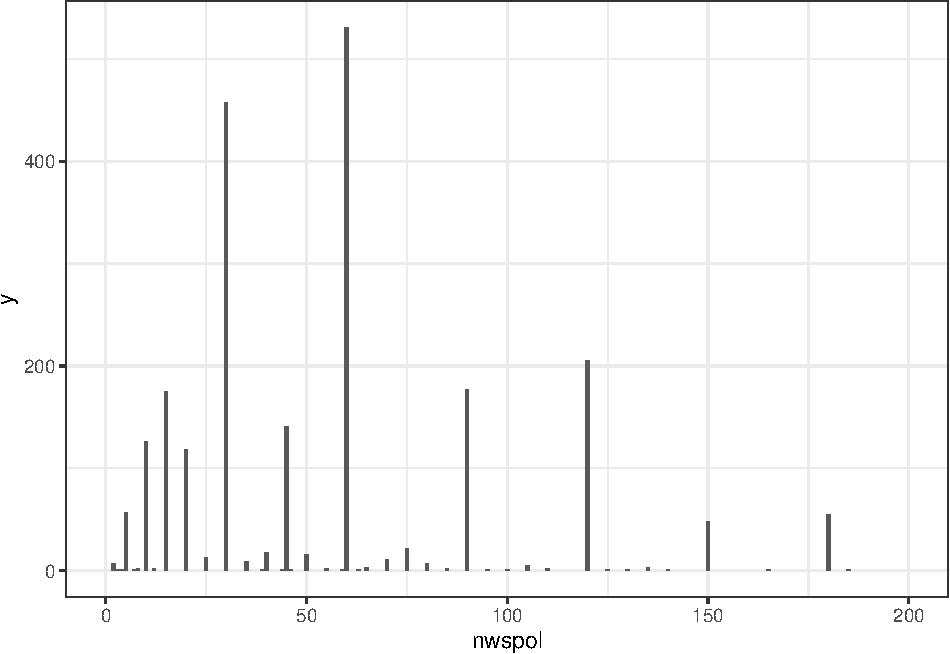
\includegraphics{ESS_DE_files/figure-latex/unnamed-chunk-4-1.pdf}

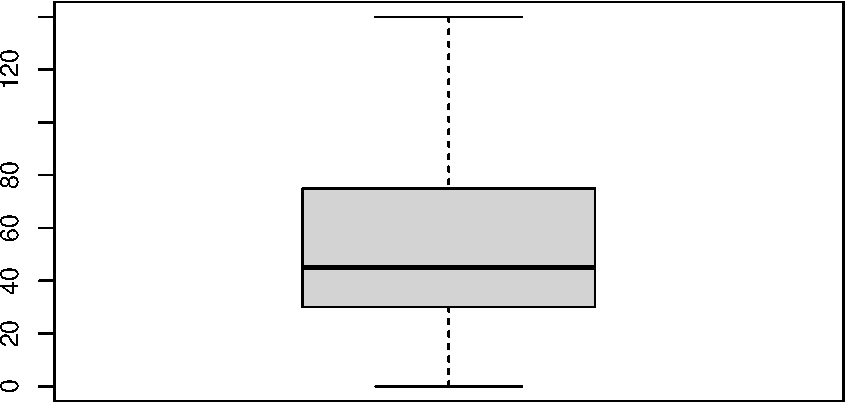
\includegraphics{ESS_DE_files/figure-latex/unnamed-chunk-5-1.pdf}

\hypertarget{was-muss-man-alles-fuxfcr-eine-deskriptive-analyse-machen}{%
\subsubsection{\texorpdfstring{\textbf{Was muss man alles für eine
deskriptive Analyse
machen?}}{Was muss man alles für eine deskriptive Analyse machen?}}\label{was-muss-man-alles-fuxfcr-eine-deskriptive-analyse-machen}}

\begin{verbatim}
## [1] "double"
\end{verbatim}

\begin{verbatim}
##    Min. 1st Qu.  Median    Mean 3rd Qu.    Max. 
##       0       0       6      43       7    8888
\end{verbatim}

\begin{verbatim}
## [1] 0
\end{verbatim}

\hypertarget{models}{%
\section{3. Models}\label{models}}

\hypertarget{linear-model}{%
\subsection{3.1 Linear Model}\label{linear-model}}

How much politics are you watching = DV\\
education level by years = IV\\
happy with government = IV\\
Gender = IV\\
Age = IV

\begin{verbatim}
## 
## Call:
## lm(formula = nwspol ~ eduade3, data = ess9_de)
## 
## Residuals:
##    Min     1Q Median     3Q    Max 
## -974.4  -33.4  -17.2   11.6 7883.6 
## 
## Coefficients:
##              Estimate Std. Error t value Pr(>|t|)    
## (Intercept) 62.165563   3.919430   15.86   <2e-16 ***
## eduade3      0.106014   0.006964   15.22   <2e-16 ***
## ---
## Signif. codes:  0 '***' 0.001 '**' 0.01 '*' 0.05 '.' 0.1 ' ' 1
## 
## Residual standard error: 189.8 on 2356 degrees of freedom
## Multiple R-squared:  0.08955,    Adjusted R-squared:  0.08916 
## F-statistic: 231.7 on 1 and 2356 DF,  p-value: < 2.2e-16
\end{verbatim}

\hypertarget{glm-poisson}{%
\subsection{3.2 GLM Poisson}\label{glm-poisson}}

The goal of this chapter is to apply a generalized linear model of the
poisson type on the ESS9 data set. The poisson model is applied to count
data, in this case the information of how many minutes the participants
spend per day for consuming media, such as newspaper, TV new shows or
online resources. In this chapter the model is used to simulate the
data, based on the provided data from the survey. First the data is
cleaned and prepared for using it. A subset of the data is used,
containing variables which should help to model the news consumption of
a person. These parameters are used: Depended variable: * How much
politics are you watching (``nwspol'') Independent variables:

\begin{itemize}
\tightlist
\item
  Interest in politics (``polintr)
\item
  Trust into the current parlament (``trstprl'')
\item
  Highest level of education (``eisced'')
\item
  Years of education (``eduyrs'')
\item
  Satisfaction with the general economical situation (``stfeco'')
\item
  Satisfaction with the current government (``stfgov'')
\item
  Gender (``gndr'')
\item
  Age (``agea'')
\item
  Level of person religion believe (``rlgdgr'')
\item
  Time spent online (``netusoft'')
\item
  Posibility for political participation (``psppsgva'')
\item
  Yearly gross income (combination of two factors into a new one -
  ``yrpy'')
\end{itemize}

\hypertarget{data-preparation}{%
\subsubsection{3.2.1 Data preparation}\label{data-preparation}}

The data have to be prepared and transformed. For poisson count data are
needed for the predictive variable. The time in minutes is modeled
therefore.

\begin{verbatim}
## [1] 572
\end{verbatim}

\begin{verbatim}
## [1] 708
\end{verbatim}

\begin{verbatim}
## [1] 1752
\end{verbatim}

\begin{verbatim}
## [1] 47
\end{verbatim}

Subset of data for this task, as 14 parameters in total. The rows with
NA are dropped, as the data set is large enough for droping theses
values.

\begin{verbatim}
## tibble [17,029 x 14] (S3: tbl_df/tbl/data.frame)
##  $ nwspol  : num [1:17029] 60 45 60 120 15 60 30 30 10 10 ...
##  $ polintr : Factor w/ 4 levels "1","2","3","4": 4 3 4 2 4 1 2 3 2 2 ...
##  $ trstprl : Factor w/ 11 levels "0","1","2","3",..: 7 1 1 7 5 4 4 8 8 6 ...
##  $ eisced  : Factor w/ 8 levels "1","2","3","4",..: 2 3 3 3 3 4 3 6 2 7 ...
##  $ eduyrs  : num [1:17029] 12 11 12 12 13 21 18 17 9 17 ...
##  $ stfeco  : Factor w/ 11 levels "0","1","2","3",..: 6 7 2 11 10 8 7 8 7 9 ...
##  $ stfgov  : Factor w/ 11 levels "0","1","2","3",..: 7 9 4 11 9 3 8 3 8 7 ...
##  $ stfdem  : Factor w/ 11 levels "0","1","2","3",..: 7 7 4 11 8 4 11 7 9 8 ...
##  $ gndr    : Factor w/ 2 levels "1","2": 2 1 1 1 2 1 1 1 1 1 ...
##  $ agea    : num [1:17029] 40 63 56 48 41 27 49 42 50 35 ...
##  $ rlgdgr  : Factor w/ 11 levels "0","1","2","3",..: 5 2 9 1 4 4 3 1 4 3 ...
##  $ netusoft: Factor w/ 5 levels "1","2","3","4",..: 4 5 1 1 4 5 5 5 5 5 ...
##  $ psppsgva: Factor w/ 5 levels "1","2","3","4",..: 2 2 2 5 1 3 1 1 2 3 ...
##  $ yrpy    : num [1:17029] 31200 30600 18000 31200 37200 18000 20400 17400 45600 70000 ...
\end{verbatim}

The plot shows the media consumption for male and female. Males have a
higher mean and the variance of the first and third quantile are larger.
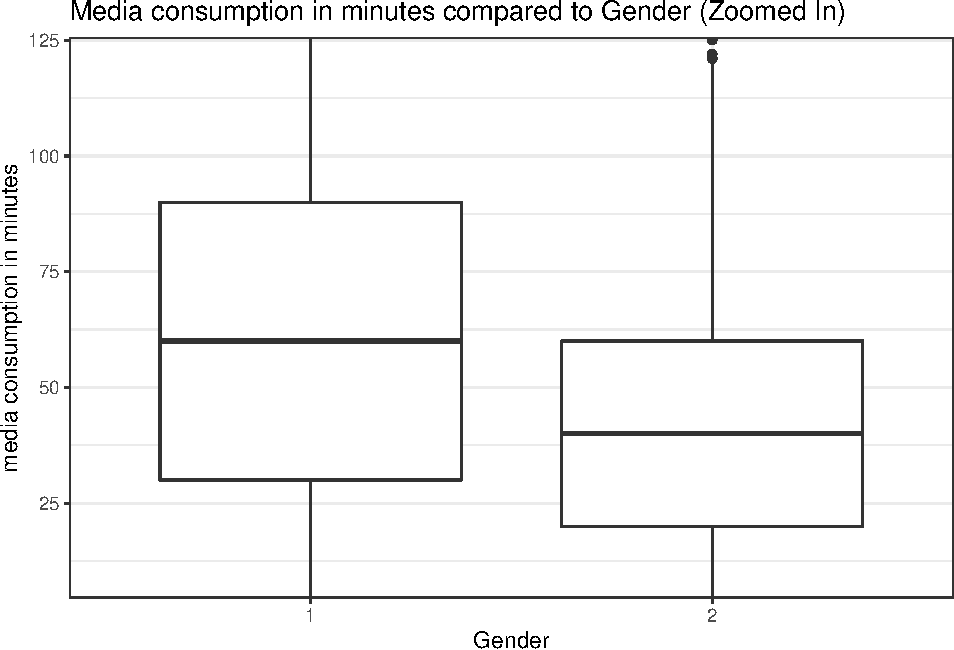
\includegraphics{ESS_DE_files/figure-latex/plotting of media consumaption-1.pdf}

\hypertarget{fitting-the-poisson-model}{%
\subsubsection{3.2.2 Fitting the poisson
model}\label{fitting-the-poisson-model}}

Using the parameter specified above to model the consumption.

\begin{verbatim}
## 
## Call:
## glm(formula = nwspol ~ polintr + eisced + trstprl + eduyrs + 
##     netusoft + stfeco + stfgov + stfdem + gndr + agea + rlgdgr + 
##     yrpy, family = "poisson", data = ess9_poisson)
## 
## Deviance Residuals: 
##     Min       1Q   Median       3Q      Max  
## -17.160   -6.476   -3.322    0.474   74.725  
## 
## Coefficients:
##               Estimate Std. Error  z value Pr(>|z|)    
## (Intercept)  4.955e+00  1.053e-02  470.379  < 2e-16 ***
## polintr2    -3.493e-01  2.668e-03 -130.918  < 2e-16 ***
## polintr3    -5.377e-01  2.882e-03 -186.586  < 2e-16 ***
## polintr4    -6.563e-01  3.735e-03 -175.697  < 2e-16 ***
## eisced2     -1.458e-01  6.474e-03  -22.524  < 2e-16 ***
## eisced3     -2.099e-01  6.390e-03  -32.847  < 2e-16 ***
## eisced4     -8.012e-02  6.296e-03  -12.725  < 2e-16 ***
## eisced5     -1.794e-01  6.604e-03  -27.163  < 2e-16 ***
## eisced6     -1.366e-02  6.805e-03   -2.007   0.0447 *  
## eisced7     -7.476e-02  7.031e-03  -10.633  < 2e-16 ***
## eisced55     1.992e-01  1.843e-02   10.805  < 2e-16 ***
## trstprl1     4.381e-02  5.642e-03    7.765 8.16e-15 ***
## trstprl2     8.788e-02  5.035e-03   17.454  < 2e-16 ***
## trstprl3     5.760e-02  4.923e-03   11.701  < 2e-16 ***
## trstprl4     1.650e-01  4.962e-03   33.249  < 2e-16 ***
## trstprl5     1.785e-01  4.696e-03   38.018  < 2e-16 ***
## trstprl6     9.264e-02  5.027e-03   18.427  < 2e-16 ***
## trstprl7     1.654e-01  5.017e-03   32.977  < 2e-16 ***
## trstprl8     2.017e-01  5.331e-03   37.839  < 2e-16 ***
## trstprl9     1.425e-01  6.802e-03   20.957  < 2e-16 ***
## trstprl10    1.035e-01  8.016e-03   12.912  < 2e-16 ***
## eduyrs      -4.784e-03  3.248e-04  -14.727  < 2e-16 ***
## netusoft2   -1.308e-01  6.282e-03  -20.817  < 2e-16 ***
## netusoft3   -1.125e-01  6.105e-03  -18.422  < 2e-16 ***
## netusoft4   -1.651e-01  5.391e-03  -30.617  < 2e-16 ***
## netusoft5   -2.565e-01  4.712e-03  -54.446  < 2e-16 ***
## stfeco1      2.043e-01  7.868e-03   25.960  < 2e-16 ***
## stfeco2      1.455e-01  6.588e-03   22.082  < 2e-16 ***
## stfeco3      1.098e-01  6.354e-03   17.275  < 2e-16 ***
## stfeco4      1.174e-01  6.396e-03   18.356  < 2e-16 ***
## stfeco5      1.061e-01  6.250e-03   16.970  < 2e-16 ***
## stfeco6      4.550e-02  6.391e-03    7.119 1.09e-12 ***
## stfeco7     -6.959e-02  6.396e-03  -10.879  < 2e-16 ***
## stfeco8     -8.449e-02  6.523e-03  -12.952  < 2e-16 ***
## stfeco9     -1.060e-01  7.320e-03  -14.481  < 2e-16 ***
## stfeco10    -2.077e-01  8.711e-03  -23.848  < 2e-16 ***
## stfgov1     -3.713e-02  5.391e-03   -6.887 5.69e-12 ***
## stfgov2     -1.629e-01  5.030e-03  -32.383  < 2e-16 ***
## stfgov3     -1.493e-01  4.958e-03  -30.103  < 2e-16 ***
## stfgov4     -8.427e-02  5.066e-03  -16.636  < 2e-16 ***
## stfgov5     -5.323e-02  4.939e-03  -10.777  < 2e-16 ***
## stfgov6     -1.646e-01  5.220e-03  -31.534  < 2e-16 ***
## stfgov7     -6.015e-02  5.289e-03  -11.373  < 2e-16 ***
## stfgov8     -1.258e-01  5.985e-03  -21.016  < 2e-16 ***
## stfgov9      1.019e-01  8.052e-03   12.652  < 2e-16 ***
## stfgov10     7.824e-02  9.832e-03    7.958 1.75e-15 ***
## stfdem1     -5.631e-02  6.911e-03   -8.147 3.72e-16 ***
## stfdem2     -2.514e-03  6.105e-03   -0.412   0.6805    
## stfdem3     -1.750e-01  6.070e-03  -28.823  < 2e-16 ***
## stfdem4     -8.346e-02  6.134e-03  -13.606  < 2e-16 ***
## stfdem5     -7.455e-02  5.907e-03  -12.621  < 2e-16 ***
## stfdem6     -1.143e-01  6.122e-03  -18.668  < 2e-16 ***
## stfdem7     -7.579e-02  6.043e-03  -12.543  < 2e-16 ***
## stfdem8     -1.282e-01  6.202e-03  -20.667  < 2e-16 ***
## stfdem9     -1.819e-01  6.948e-03  -26.184  < 2e-16 ***
## stfdem10    -1.082e-01  7.980e-03  -13.555  < 2e-16 ***
## gndr2       -9.552e-02  1.893e-03  -50.466  < 2e-16 ***
## agea         3.944e-03  7.526e-05   52.407  < 2e-16 ***
## rlgdgr1      5.246e-02  3.913e-03   13.407  < 2e-16 ***
## rlgdgr2      2.296e-02  3.716e-03    6.178 6.50e-10 ***
## rlgdgr3      1.252e-01  3.590e-03   34.881  < 2e-16 ***
## rlgdgr4      9.111e-02  4.047e-03   22.511  < 2e-16 ***
## rlgdgr5      8.948e-04  3.270e-03    0.274   0.7844    
## rlgdgr6      5.993e-02  3.589e-03   16.698  < 2e-16 ***
## rlgdgr7     -7.732e-03  3.578e-03   -2.161   0.0307 *  
## rlgdgr8      7.930e-03  3.853e-03    2.058   0.0396 *  
## rlgdgr9     -7.510e-02  5.968e-03  -12.584  < 2e-16 ***
## rlgdgr10     1.758e-01  4.737e-03   37.114  < 2e-16 ***
## yrpy        -8.538e-09  5.367e-10  -15.907  < 2e-16 ***
## ---
## Signif. codes:  0 '***' 0.001 '**' 0.01 '*' 0.05 '.' 0.1 ' ' 1
## 
## (Dispersion parameter for poisson family taken to be 1)
## 
##     Null deviance: 1622523  on 17028  degrees of freedom
## Residual deviance: 1532064  on 16960  degrees of freedom
## AIC: 1622455
## 
## Number of Fisher Scoring iterations: 6
\end{verbatim}

\begin{verbatim}
##   (Intercept)      polintr2      polintr3      polintr4       eisced2 
##  4.955148e+00 -3.492666e-01 -5.376727e-01 -6.563093e-01 -1.458106e-01 
##       eisced3       eisced4       eisced5       eisced6       eisced7 
## -2.098897e-01 -8.011801e-02 -1.793752e-01 -1.365827e-02 -7.476229e-02 
##      eisced55      trstprl1      trstprl2      trstprl3      trstprl4 
##  1.991819e-01  4.381167e-02  8.787872e-02  5.759928e-02  1.649700e-01 
##      trstprl5      trstprl6      trstprl7      trstprl8      trstprl9 
##  1.785394e-01  9.264118e-02  1.654323e-01  2.017014e-01  1.425489e-01 
##     trstprl10        eduyrs     netusoft2     netusoft3     netusoft4 
##  1.034980e-01 -4.783826e-03 -1.307787e-01 -1.124714e-01 -1.650625e-01 
##     netusoft5       stfeco1       stfeco2       stfeco3       stfeco4 
## -2.565500e-01  2.042630e-01  1.454845e-01  1.097594e-01  1.173994e-01 
##       stfeco5       stfeco6       stfeco7       stfeco8       stfeco9 
##  1.060677e-01  4.549509e-02 -6.958551e-02 -8.448505e-02 -1.059951e-01 
##      stfeco10       stfgov1       stfgov2       stfgov3       stfgov4 
## -2.077250e-01 -3.712830e-02 -1.628748e-01 -1.492579e-01 -8.427065e-02 
##       stfgov5       stfgov6       stfgov7       stfgov8       stfgov9 
## -5.322969e-02 -1.646096e-01 -6.014933e-02 -1.257886e-01  1.018728e-01 
##      stfgov10       stfdem1       stfdem2       stfdem3       stfdem4 
##  7.824075e-02 -5.630986e-02 -2.513800e-03 -1.749548e-01 -8.345531e-02 
##       stfdem5       stfdem6       stfdem7       stfdem8       stfdem9 
## -7.455110e-02 -1.142835e-01 -7.579213e-02 -1.281855e-01 -1.819244e-01 
##      stfdem10         gndr2          agea       rlgdgr1       rlgdgr2 
## -1.081689e-01 -9.552218e-02  3.944284e-03  5.245943e-02  2.295902e-02 
##       rlgdgr3       rlgdgr4       rlgdgr5       rlgdgr6       rlgdgr7 
##  1.252369e-01  9.110513e-02  8.947887e-04  5.993445e-02 -7.731684e-03 
##       rlgdgr8       rlgdgr9      rlgdgr10          yrpy 
##  7.929514e-03 -7.509784e-02  1.758154e-01 -8.538016e-09
\end{verbatim}

\begin{verbatim}
## (Intercept) 
##    141.9036
\end{verbatim}

\hypertarget{simulation}{%
\subsubsection{3.2.3 Simulation}\label{simulation}}

Now we simulate with our model the average media consumption for Females
and Males.

\begin{verbatim}
## [1] 17029
\end{verbatim}

\begin{verbatim}
##   sim_1
## 1    48
## 2    47
## 3    53
## 4    81
## 5    44
## 6    79
\end{verbatim}

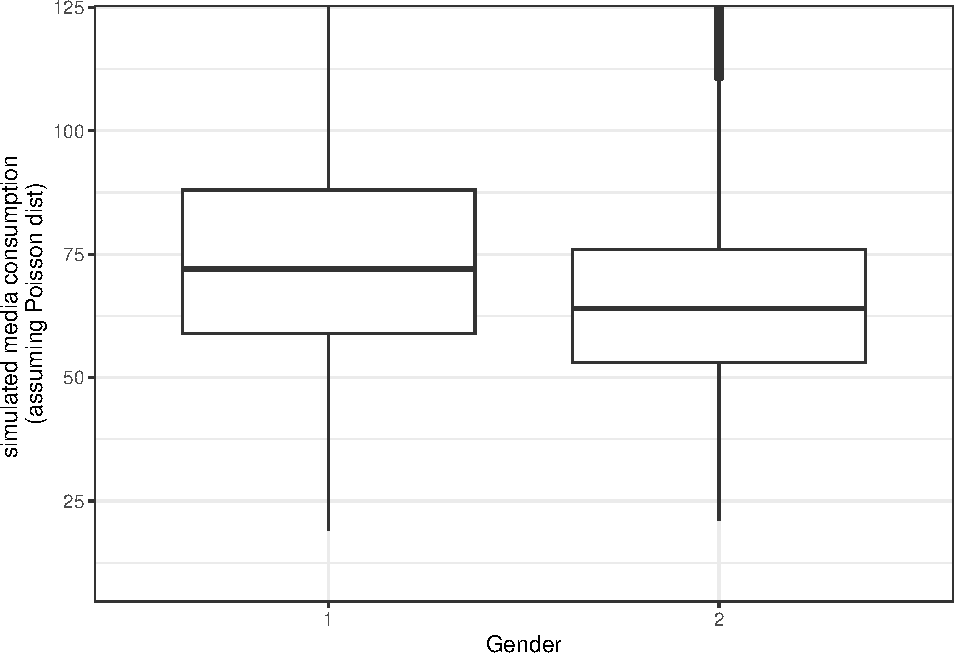
\includegraphics{ESS_DE_files/figure-latex/poisson simulation of data-1.pdf}
The simulated data look similar as the real data based of the survey.
The variance is smaller for the simulated one. The higher mean and the
higher variance for the male group is indicated in the real data as well
as in the simulated data.

\hypertarget{glm-quasi-poisson}{%
\subsubsection{3.2.4 GLM Quasi-Poisson}\label{glm-quasi-poisson}}

\begin{verbatim}
## 
## Call:
## glm(formula = nwspol ~ polintr + eisced + trstprl + eduyrs + 
##     netusoft + stfeco + stfgov + stfdem + gndr + agea + rlgdgr + 
##     yrpy, family = "quasipoisson", data = ess9_poisson)
## 
## Deviance Residuals: 
##     Min       1Q   Median       3Q      Max  
## -17.160   -6.476   -3.322    0.474   74.725  
## 
## Coefficients:
##               Estimate Std. Error t value Pr(>|t|)    
## (Intercept)  4.955e+00  1.513e-01  32.746  < 2e-16 ***
## polintr2    -3.493e-01  3.832e-02  -9.114  < 2e-16 ***
## polintr3    -5.377e-01  4.139e-02 -12.990  < 2e-16 ***
## polintr4    -6.563e-01  5.366e-02 -12.232  < 2e-16 ***
## eisced2     -1.458e-01  9.299e-02  -1.568 0.116894    
## eisced3     -2.099e-01  9.179e-02  -2.287 0.022227 *  
## eisced4     -8.012e-02  9.044e-02  -0.886 0.375685    
## eisced5     -1.794e-01  9.486e-02  -1.891 0.058638 .  
## eisced6     -1.366e-02  9.775e-02  -0.140 0.888873    
## eisced7     -7.476e-02  1.010e-01  -0.740 0.459160    
## eisced55     1.992e-01  2.648e-01   0.752 0.451927    
## trstprl1     4.381e-02  8.105e-02   0.541 0.588802    
## trstprl2     8.788e-02  7.232e-02   1.215 0.224347    
## trstprl3     5.760e-02  7.071e-02   0.815 0.415319    
## trstprl4     1.650e-01  7.127e-02   2.315 0.020643 *  
## trstprl5     1.785e-01  6.746e-02   2.647 0.008136 ** 
## trstprl6     9.264e-02  7.222e-02   1.283 0.199568    
## trstprl7     1.654e-01  7.206e-02   2.296 0.021703 *  
## trstprl8     2.017e-01  7.657e-02   2.634 0.008440 ** 
## trstprl9     1.425e-01  9.771e-02   1.459 0.144599    
## trstprl10    1.035e-01  1.151e-01   0.899 0.368720    
## eduyrs      -4.784e-03  4.666e-03  -1.025 0.305273    
## netusoft2   -1.308e-01  9.024e-02  -1.449 0.147299    
## netusoft3   -1.125e-01  8.770e-02  -1.283 0.199682    
## netusoft4   -1.651e-01  7.744e-02  -2.131 0.033063 *  
## netusoft5   -2.565e-01  6.768e-02  -3.790 0.000151 ***
## stfeco1      2.043e-01  1.130e-01   1.807 0.070742 .  
## stfeco2      1.455e-01  9.464e-02   1.537 0.124234    
## stfeco3      1.098e-01  9.127e-02   1.203 0.229140    
## stfeco4      1.174e-01  9.187e-02   1.278 0.201304    
## stfeco5      1.061e-01  8.978e-02   1.181 0.237464    
## stfeco6      4.550e-02  9.180e-02   0.496 0.620187    
## stfeco7     -6.959e-02  9.187e-02  -0.757 0.448823    
## stfeco8     -8.449e-02  9.370e-02  -0.902 0.367257    
## stfeco9     -1.060e-01  1.051e-01  -1.008 0.313419    
## stfeco10    -2.077e-01  1.251e-01  -1.660 0.096893 .  
## stfgov1     -3.713e-02  7.744e-02  -0.479 0.631617    
## stfgov2     -1.629e-01  7.225e-02  -2.254 0.024185 *  
## stfgov3     -1.493e-01  7.122e-02  -2.096 0.036124 *  
## stfgov4     -8.427e-02  7.277e-02  -1.158 0.246833    
## stfgov5     -5.323e-02  7.095e-02  -0.750 0.453093    
## stfgov6     -1.646e-01  7.498e-02  -2.195 0.028154 *  
## stfgov7     -6.015e-02  7.597e-02  -0.792 0.428511    
## stfgov8     -1.258e-01  8.598e-02  -1.463 0.143474    
## stfgov9      1.019e-01  1.157e-01   0.881 0.378443    
## stfgov10     7.824e-02  1.412e-01   0.554 0.579573    
## stfdem1     -5.631e-02  9.928e-02  -0.567 0.570587    
## stfdem2     -2.514e-03  8.769e-02  -0.029 0.977130    
## stfdem3     -1.750e-01  8.719e-02  -2.007 0.044809 *  
## stfdem4     -8.346e-02  8.811e-02  -0.947 0.343542    
## stfdem5     -7.455e-02  8.485e-02  -0.879 0.379625    
## stfdem6     -1.143e-01  8.794e-02  -1.300 0.193757    
## stfdem7     -7.579e-02  8.680e-02  -0.873 0.382571    
## stfdem8     -1.282e-01  8.909e-02  -1.439 0.150234    
## stfdem9     -1.819e-01  9.980e-02  -1.823 0.068344 .  
## stfdem10    -1.082e-01  1.146e-01  -0.944 0.345374    
## gndr2       -9.552e-02  2.719e-02  -3.513 0.000444 ***
## agea         3.944e-03  1.081e-03   3.648 0.000265 ***
## rlgdgr1      5.246e-02  5.621e-02   0.933 0.350665    
## rlgdgr2      2.296e-02  5.338e-02   0.430 0.667145    
## rlgdgr3      1.252e-01  5.157e-02   2.428 0.015180 *  
## rlgdgr4      9.111e-02  5.813e-02   1.567 0.117099    
## rlgdgr5      8.948e-04  4.697e-02   0.019 0.984801    
## rlgdgr6      5.993e-02  5.156e-02   1.162 0.245063    
## rlgdgr7     -7.732e-03  5.140e-02  -0.150 0.880431    
## rlgdgr8      7.930e-03  5.534e-02   0.143 0.886069    
## rlgdgr9     -7.510e-02  8.572e-02  -0.876 0.381007    
## rlgdgr10     1.758e-01  6.805e-02   2.584 0.009780 ** 
## yrpy        -8.538e-09  7.710e-09  -1.107 0.268132    
## ---
## Signif. codes:  0 '***' 0.001 '**' 0.01 '*' 0.05 '.' 0.1 ' ' 1
## 
## (Dispersion parameter for quasipoisson family taken to be 206.3327)
## 
##     Null deviance: 1622523  on 17028  degrees of freedom
## Residual deviance: 1532064  on 16960  degrees of freedom
## AIC: NA
## 
## Number of Fisher Scoring iterations: 6
\end{verbatim}

\begin{verbatim}
## Analysis of Deviance Table
## 
## Model 1: nwspol ~ polintr + eisced + trstprl + eduyrs + netusoft + stfeco + 
##     stfgov + stfdem + gndr + agea + rlgdgr + yrpy
## Model 2: nwspol ~ polintr + eisced + trstprl + eduyrs + netusoft + stfeco + 
##     stfgov + stfdem + agea + rlgdgr + yrpy
##   Resid. Df Resid. Dev Df Deviance     F    Pr(>F)    
## 1     16960    1532064                                
## 2     16961    1534617 -1  -2552.4 12.37 0.0004373 ***
## ---
## Signif. codes:  0 '***' 0.001 '**' 0.01 '*' 0.05 '.' 0.1 ' ' 1
\end{verbatim}

Yes, Gender plays a role for the quasi poisson model.

\begin{verbatim}
## Analysis of Deviance Table
## 
## Model 1: nwspol ~ polintr + eisced + trstprl + eduyrs + netusoft + stfeco + 
##     stfgov + stfdem + gndr + agea + rlgdgr + yrpy
## Model 2: nwspol ~ polintr + eisced + trstprl + eduyrs + netusoft + stfeco + 
##     stfgov + gndr + agea + rlgdgr + yrpy
##   Resid. Df Resid. Dev  Df Deviance      F Pr(>F)
## 1     16960    1532064                           
## 2     16970    1534358 -10  -2293.3 1.1114 0.3488
\end{verbatim}

To compare it with the variable of ``stfdem'' about how satisfied the
participants of the survey are about how the democracy in their country
works. This variable doensn't play a role to predict the media
consumption according to the quasipoisson model.

\hypertarget{labs-example}{%
\subsubsection{Labs Example}\label{labs-example}}

\textless\textless\textless\textless\textless\textless\textless{}
HEAD:ESS9.csv/ESS\_DE.Rmd \#\# 3.3 GLM Binominal =======

\hypertarget{glm-binominal}{%
\subsection{3.3 GLM Binominal}\label{glm-binominal}}

\begin{quote}
\begin{quote}
\begin{quote}
\begin{quote}
\begin{quote}
\begin{quote}
\begin{quote}
d33abb64bd4520b2c184cf8af74b866bfe227af9:ESS9.csv/rfile/ESS\_DE.Rmd
\end{quote}
\end{quote}
\end{quote}
\end{quote}
\end{quote}
\end{quote}
\end{quote}

\hypertarget{gam}{%
\subsection{3.4 GAM}\label{gam}}

In this chapter a generalized additive model (GAM) is applied to the
data set. First the data is visually analyzed and checked. The variables
don't show a strong relation ship and the line is mostly horizontal.

\includegraphics{ESS_DE_files/figure-latex/GAM peperation-1.pdf}
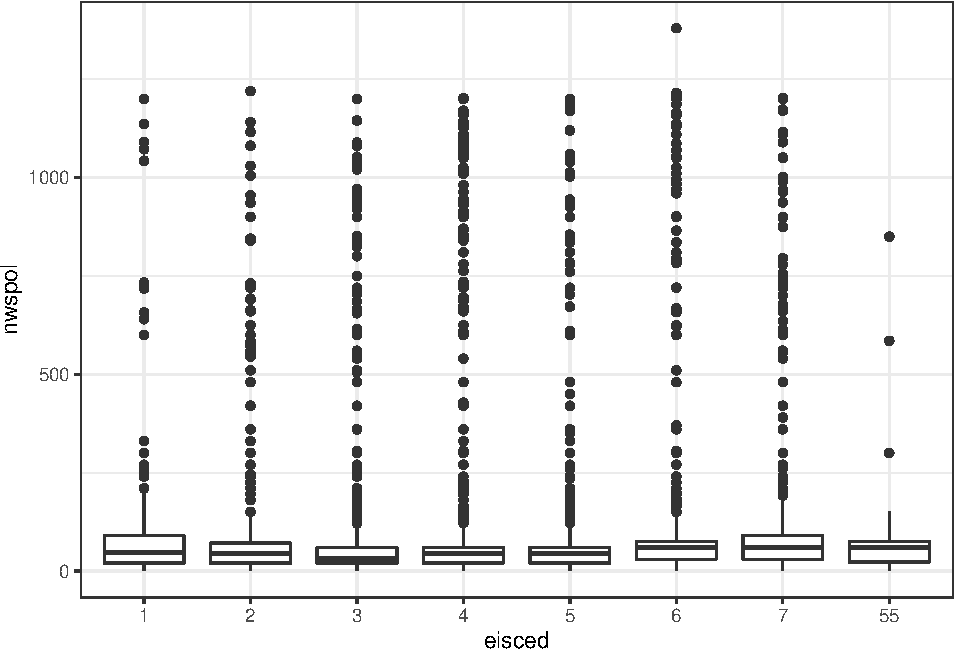
\includegraphics{ESS_DE_files/figure-latex/GAM peperation-2.pdf}
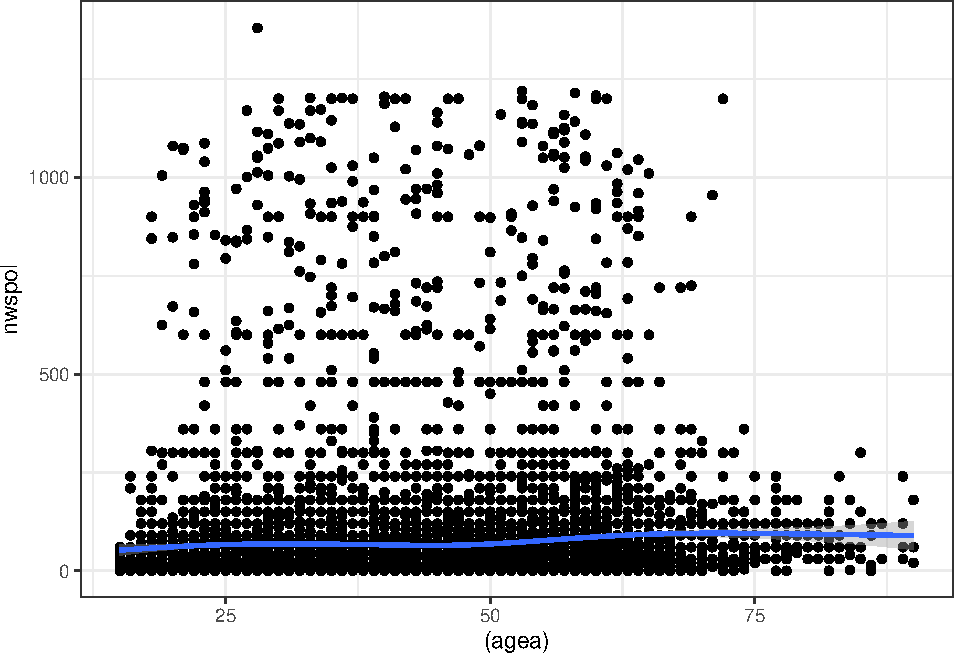
\includegraphics{ESS_DE_files/figure-latex/GAM peperation-3.pdf}
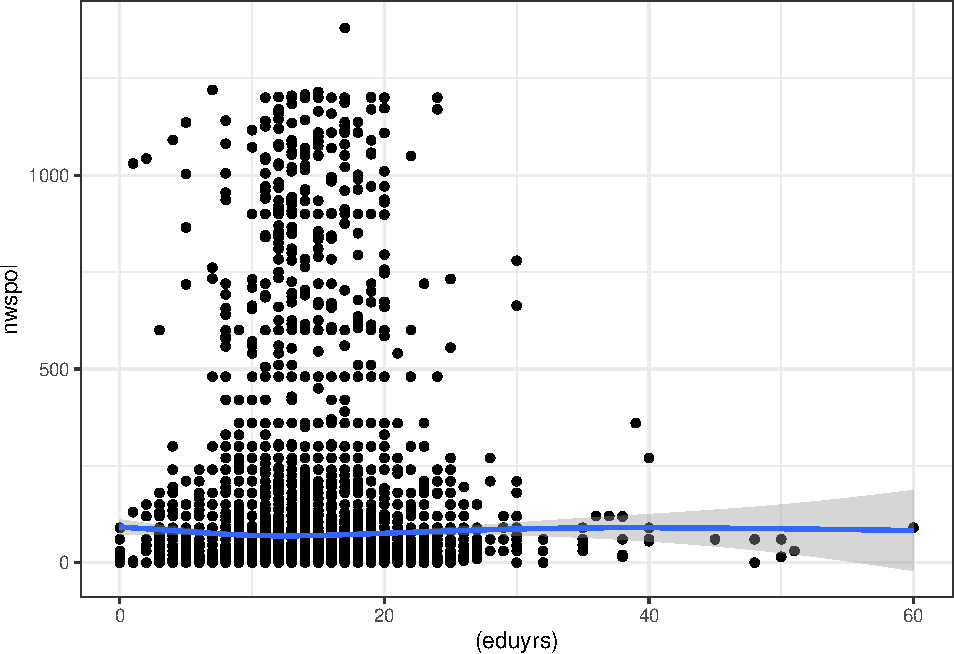
\includegraphics{ESS_DE_files/figure-latex/GAM peperation-4.pdf}
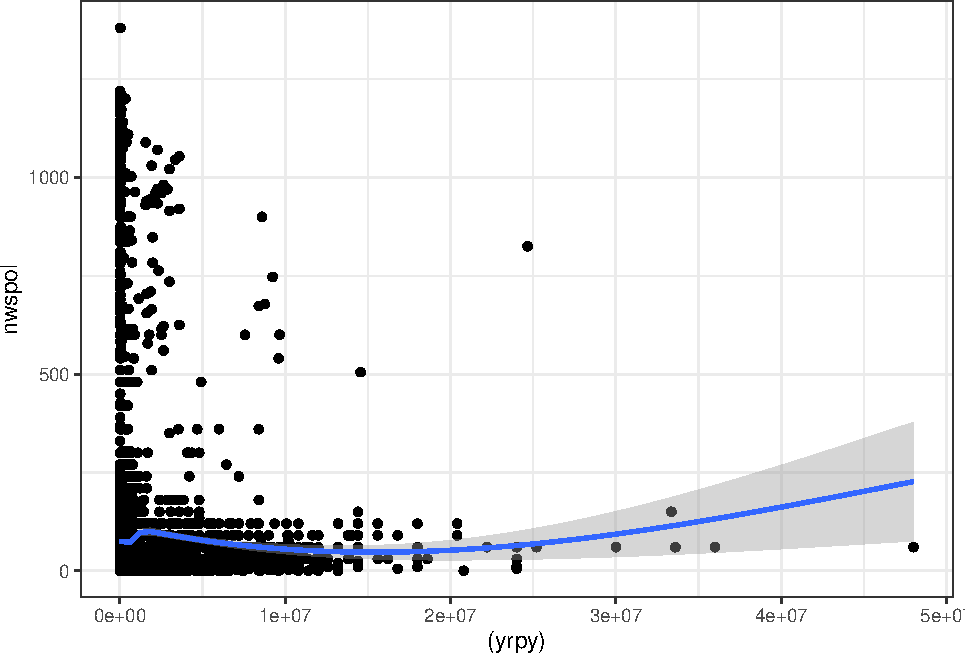
\includegraphics{ESS_DE_files/figure-latex/GAM peperation-5.pdf}

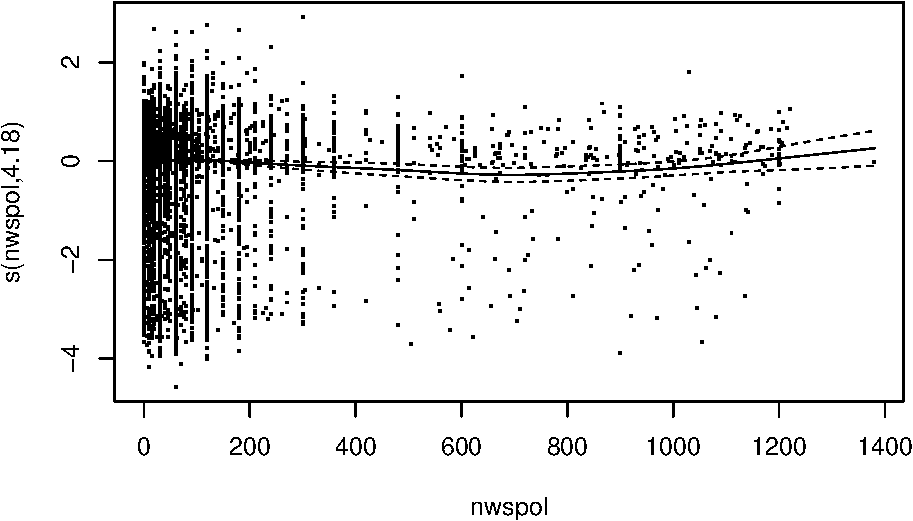
\includegraphics{ESS_DE_files/figure-latex/GAM-1.pdf}
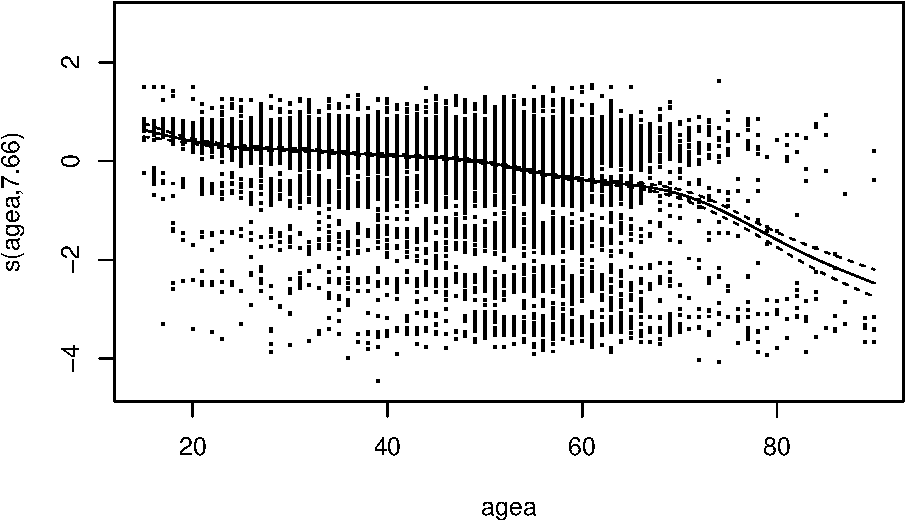
\includegraphics{ESS_DE_files/figure-latex/GAM-2.pdf}
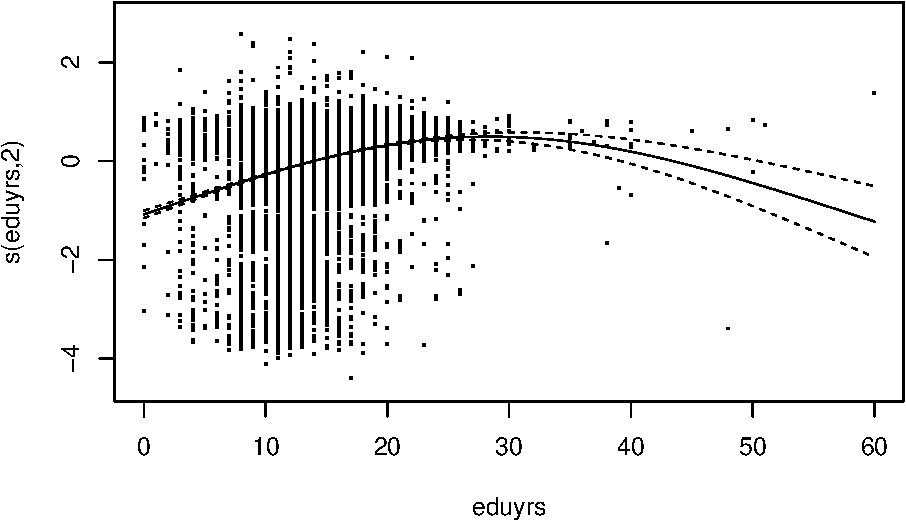
\includegraphics{ESS_DE_files/figure-latex/GAM-3.pdf}
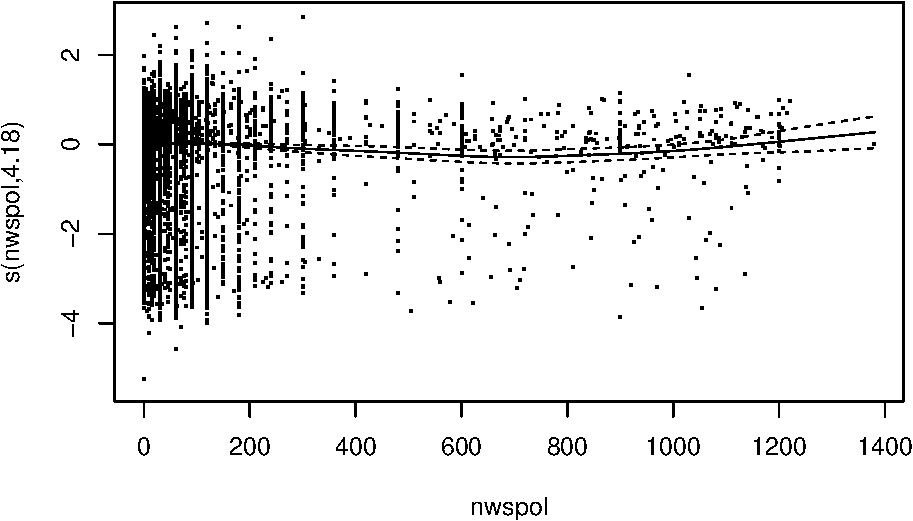
\includegraphics{ESS_DE_files/figure-latex/unnamed-chunk-8-1.pdf}
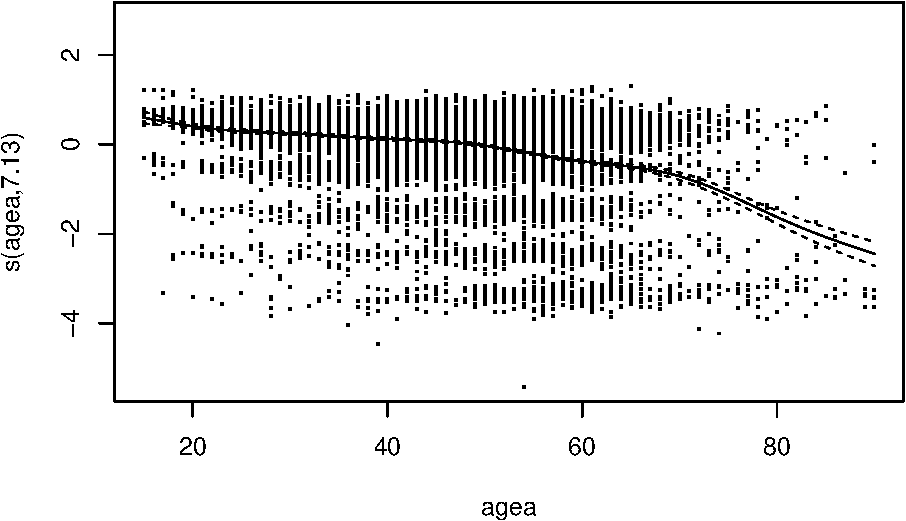
\includegraphics{ESS_DE_files/figure-latex/unnamed-chunk-8-2.pdf}

\hypertarget{neural-network}{%
\subsection{3.5 Neural Network}\label{neural-network}}

Within this chapter two types of neural network model are applied to two
different questions.

\begin{enumerate}
\def\labelenumi{\arabic{enumi}.}
\tightlist
\item
  Predicting the values for the continuous variable
\item
  Predicting the vallues for the categorical variable inidicating the 5
  levels of \#\#\# 3.5.1 continious variable
\end{enumerate}

\begin{verbatim}
## tibble [17,029 x 14] (S3: tbl_df/tbl/data.frame)
##  $ nwspol  : num [1:17029] 60 45 60 120 15 60 30 30 10 10 ...
##  $ polintr : num [1:17029] 4 3 4 2 4 1 2 3 2 2 ...
##  $ trstprl : num [1:17029] 6 0 0 6 4 3 3 7 7 5 ...
##  $ eisced  : num [1:17029] 2 3 3 3 3 4 3 6 2 7 ...
##  $ eduyrs  : num [1:17029] 12 11 12 12 13 21 18 17 9 17 ...
##  $ stfeco  : num [1:17029] 5 6 1 10 9 7 6 7 6 8 ...
##  $ stfgov  : num [1:17029] 6 8 3 10 8 2 7 2 7 6 ...
##  $ stfdem  : num [1:17029] 6 6 3 10 7 3 10 6 8 7 ...
##  $ gndr    : num [1:17029] 2 1 1 1 2 1 1 1 1 1 ...
##  $ agea    : num [1:17029] 40 63 56 48 41 27 49 42 50 35 ...
##  $ rlgdgr  : num [1:17029] 4 1 8 0 3 3 2 0 3 2 ...
##  $ netusoft: num [1:17029] 4 5 1 1 4 5 5 5 5 5 ...
##  $ psppsgva: num [1:17029] 2 2 2 5 1 3 1 1 2 3 ...
##  $ yrpy    : num [1:17029] 31200 30600 18000 31200 37200 18000 20400 17400 45600 70000 ...
\end{verbatim}

\hypertarget{prepare-for-training}{%
\paragraph{Prepare for Training}\label{prepare-for-training}}

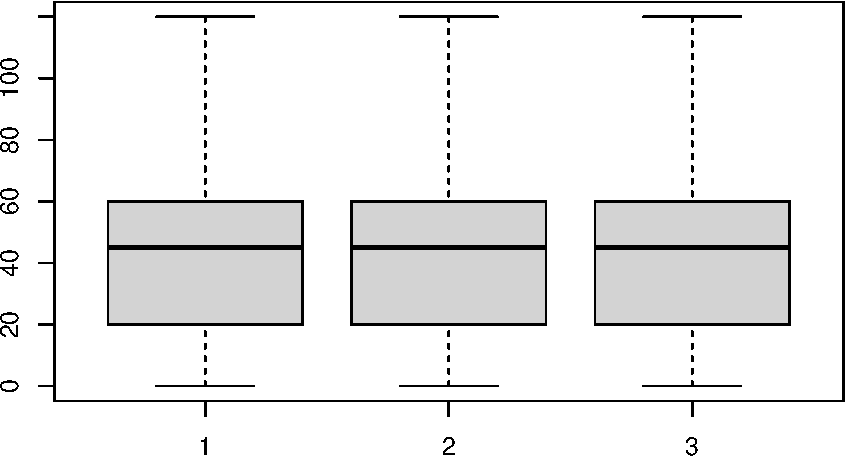
\includegraphics{ESS_DE_files/figure-latex/preparation-1.pdf}

\hypertarget{fit-the-network}{%
\paragraph{Fit the Network}\label{fit-the-network}}

\hypertarget{predict-the-test-set}{%
\paragraph{Predict the test set}\label{predict-the-test-set}}

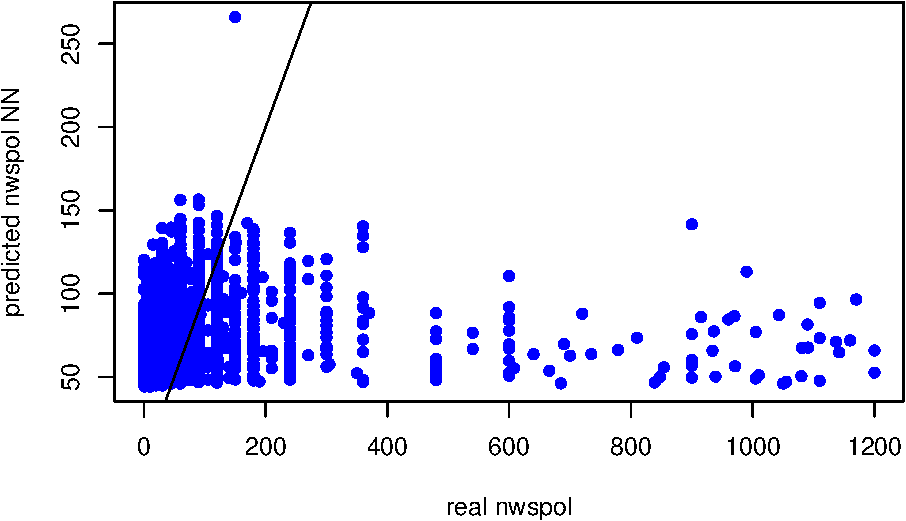
\includegraphics{ESS_DE_files/figure-latex/plot comparsion of real and predicated data-1.pdf}
And calculate the RMSE

\begin{verbatim}
## [1] 123.4398
\end{verbatim}

\hypertarget{redo-with-caret-and-cross-validation}{%
\paragraph{\texorpdfstring{Redo with \texttt{caret} and Cross
Validation}{Redo with caret and Cross Validation}}\label{redo-with-caret-and-cross-validation}}

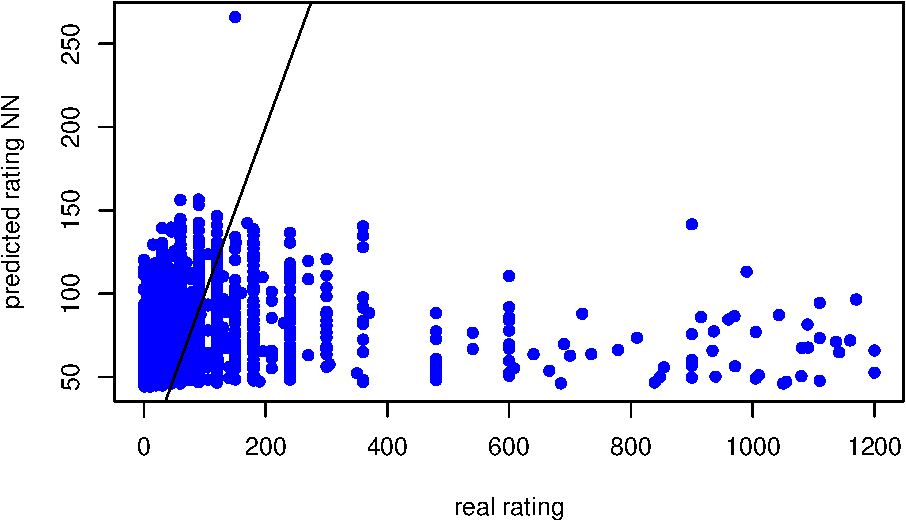
\includegraphics{ESS_DE_files/figure-latex/unnamed-chunk-9-1.pdf}

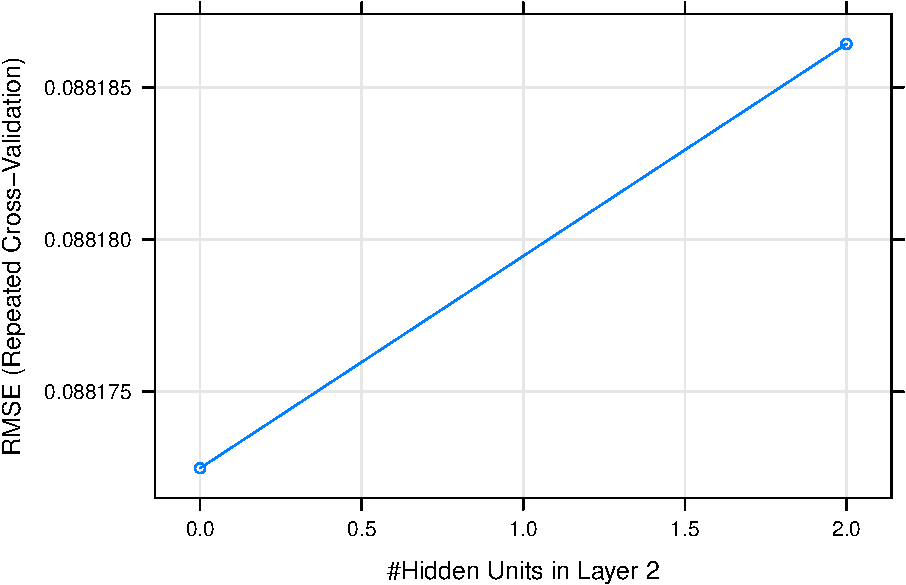
\includegraphics{ESS_DE_files/figure-latex/unnamed-chunk-10-1.pdf}

\hypertarget{categorical-variable}{%
\subsubsection{3.5.2 Categorical variable}\label{categorical-variable}}

\begin{verbatim}
## tibble [17,029 x 14] (S3: tbl_df/tbl/data.frame)
##  $ nwspol  : num [1:17029] 60 45 60 120 15 60 30 30 10 10 ...
##  $ polintr : num [1:17029] 4 3 4 2 4 1 2 3 2 2 ...
##  $ trstprl : num [1:17029] 6 0 0 6 4 3 3 7 7 5 ...
##  $ eisced  : num [1:17029] 2 3 3 3 3 4 3 6 2 7 ...
##  $ eduyrs  : num [1:17029] 12 11 12 12 13 21 18 17 9 17 ...
##  $ stfeco  : num [1:17029] 5 6 1 10 9 7 6 7 6 8 ...
##  $ stfgov  : num [1:17029] 6 8 3 10 8 2 7 2 7 6 ...
##  $ stfdem  : num [1:17029] 6 6 3 10 7 3 10 6 8 7 ...
##  $ gndr    : num [1:17029] 2 1 1 1 2 1 1 1 1 1 ...
##  $ agea    : num [1:17029] 40 63 56 48 41 27 49 42 50 35 ...
##  $ rlgdgr  : num [1:17029] 4 1 8 0 3 3 2 0 3 2 ...
##  $ netusoft: Factor w/ 5 levels "1","2","3","4",..: 4 5 1 1 4 5 5 5 5 5 ...
##  $ psppsgva: num [1:17029] 2 2 2 5 1 3 1 1 2 3 ...
##  $ yrpy    : num [1:17029] 31200 30600 18000 31200 37200 18000 20400 17400 45600 70000 ...
\end{verbatim}

\hypertarget{have-a-quick-look-at-the-data}{%
\paragraph{Have a quick look at the
Data}\label{have-a-quick-look-at-the-data}}

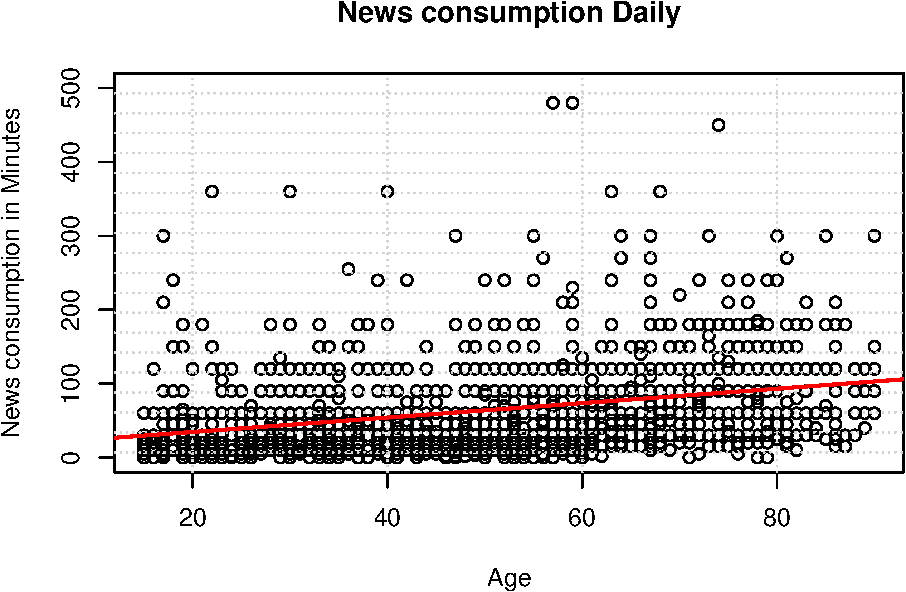
\includegraphics{ESS_DE_files/figure-latex/unnamed-chunk-12-1.pdf}

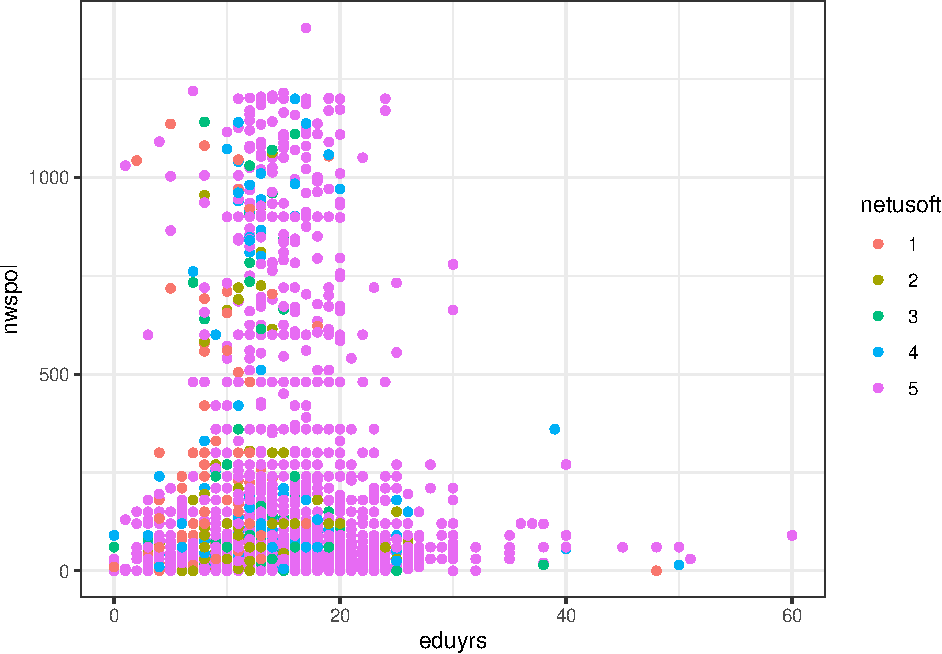
\includegraphics{ESS_DE_files/figure-latex/unnamed-chunk-13-1.pdf}

\hypertarget{prepare-the-data-for-training}{%
\paragraph{Prepare the Data for
Training}\label{prepare-the-data-for-training}}

\hypertarget{why-do-we-use-the-caret-function}{%
\paragraph{\texorpdfstring{Why do we use the \texttt{caret}
function}{Why do we use the caret function}}\label{why-do-we-use-the-caret-function}}

Look at the distribution of our different prediction classes in the
train and test datasets:

\begin{verbatim}
##         train
## netusoft FALSE  TRUE
##        1    90   515
##        2    91   516
##        3   106   604
##        4   210  1193
##        5  2055 11649
\end{verbatim}

Now compare this to the ``random'' approach:

\begin{verbatim}
##         train
## netusoft FALSE  TRUE
##        1   104   501
##        2    89   518
##        3   106   604
##        4   197  1206
##        5  2033 11671
\end{verbatim}

So using the \texttt{createDataPartition} function makes sure that no
class is over- or underrepresented relative to the total occurance in
the two sets

\hypertarget{create-some-easy-variables-to-access-data}{%
\paragraph{Create some easy Variables to access
Data}\label{create-some-easy-variables-to-access-data}}

\hypertarget{train-the-neural-network}{%
\paragraph{Train the Neural Network}\label{train-the-neural-network}}

Call the \texttt{neuralnet} function creating a network with two hidden
layers containing 4 and 3 neurons (probably way too complex for our
problem here).

Plot the resulting network including the weights

\hypertarget{make-predictions}{%
\paragraph{Make Predictions}\label{make-predictions}}

Find class (i.e.~output neuron) with the highest probability and convert
this back into a factor

\hypertarget{evaluate-the-results}{%
\paragraph{Evaluate the Results}\label{evaluate-the-results}}

\begin{verbatim}
## Confusion Matrix and Statistics
## 
##           Reference
## Prediction    1    2    3    4    5
##          1    1    0    0    0   89
##          2    0    0    0    0   91
##          3    0    0    0    0  106
##          4    0    0    0    0  210
##          5    0    0    0    0 2055
## 
## Overall Statistics
##                                           
##                Accuracy : 0.8056          
##                  95% CI : (0.7897, 0.8208)
##     No Information Rate : 0.9996          
##     P-Value [Acc > NIR] : 1               
##                                           
##                   Kappa : 0.0036          
##                                           
##  Mcnemar's Test P-Value : NA              
## 
## Statistics by Class:
## 
##                       Class: 1 Class: 2 Class: 3 Class: 4 Class: 5
## Sensitivity          1.0000000       NA       NA       NA 0.805566
## Specificity          0.9651117  0.96434  0.95846  0.91771 1.000000
## Pos Pred Value       0.0111111       NA       NA       NA 1.000000
## Neg Pred Value       1.0000000       NA       NA       NA 0.002012
## Prevalence           0.0003918  0.00000  0.00000  0.00000 0.999608
## Detection Rate       0.0003918  0.00000  0.00000  0.00000 0.805251
## Detection Prevalence 0.0352665  0.03566  0.04154  0.08229 0.805251
## Balanced Accuracy    0.9825559       NA       NA       NA 0.902783
\end{verbatim}

\hypertarget{optimize-network-structure}{%
\paragraph{Optimize Network
Structure}\label{optimize-network-structure}}

First we need to remodel the data due to some limitations of
\texttt{caret}

\begin{verbatim}
##   netusoft netusoft2 netusoft3 netusoft4 netusoft5
## 1        1         0         0         1         0
## 2        1         0         0         0         1
## 3        1         0         0         0         0
## 4        1         0         0         0         0
## 5        1         0         0         1         0
## 6        1         0         0         0         1
\end{verbatim}

And have a look at the different models

\includegraphics{ESS_DE_files/figure-latex/unnamed-chunk-22-1.pdf}

And try out the best model

\hypertarget{support-vector-machine}{%
\subsection{3.6 Support Vector Machine}\label{support-vector-machine}}

\end{document}
